%! TEX root = simbol_las.tex
% the main TeX file which is intended to compile, :VimtexReload after adjustment
   % this file should be included in the main file
% :h vimtex-tex-root
\documentclass[../menggambarteknik.tex]{subfiles}
%ensure the class of docs

\begin{document}

\section{Simbol Las}%
\label{sec:Simbol Las}

\subsection{Tujuan}%
\label{sub:Tujuan}

Setelah mempelajari bahan dalam bab ini, seharusnya Anda dapat:
\begin{itemize}
	\item Mengidentifikasi bentuk-bentuk sambungan las.
	\item Menafsirkan bentuk alur las.
	\item Membaca lambang las pada gambar kerja.
	\item Menggunakan lambang-lambang las pada gambar kerja
\end{itemize}

\subsection{Bentuk Sambungan dan Alur Las}%
\label{sub:bentuk_sambungan_dan_alur_las}

Sebagai alat penyambung yang bersifat permanen pada bagian-bagian mesin atau konstruksi, pengelasan merupakan sambungan yang lebih ringan dan kuat bila dibandingkan dengan sambungan paku keling. Kemajuan teknologi menyebabkan penggunaan penyambungan dengan las semakin luas dalam industri kecil maupun besar. Bentuk sambungan las dapat digolongkan seperti terlihat pada gambar~\ref{fig:samblas} di bawah ini.

\begin{figure}
	\begin{center}
		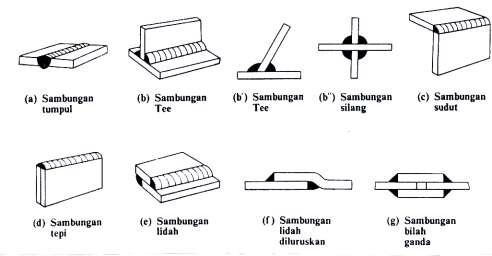
\includegraphics[width=.82\textwidth]{../figures/samb_las.jpg}
		% filename may not contain space but _
	\end{center}
	\caption{Bentuk Sambungan Las}
	\label{fig:samblas}
\end{figure}


Untuk mengisi cairan las pada benda yang akan disambung dibutuhkan alur las. Alur las inilah yang nantinya akan menyatukan benda-benda yang akan disambung. Bentuk alur las yang biasa digunakan pada sambungan las adalah seperti terlihat pada gambar~\ref{fig:alurlas} di bawah ini.

\begin{figure}
	\begin{center}
		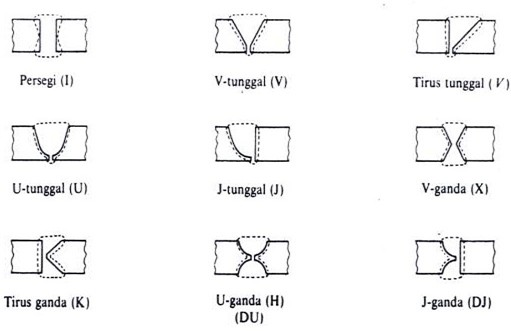
\includegraphics[width=.82\textwidth]{../figures/alur_las.jpg}
		% filename may not contain space but _
	\end{center}
	\caption{Bentuk-bentuk alur las}
	\label{fig:alurlas}
\end{figure}


\subsection{Lambang Las}%
\label{sub:lambang_las}


Perencana maupun pemesan yang menginginkan suatu bentuk pengelasan tertentu pada tukang las harus menyampaikannya dalam bentuk gambar dan dilakukan dengan bentuk-bentuk lambang khusus untuk lebih menyederhanakan gambar. Bentuk lambang yang biasa digunakan baik untuk tunggal maupun ganda (dua sisi) adalah seperti terlihat pada tabel~\ref{fig:lambang_las} di bawah ini.

\begin{figure}
	\begin{center}
		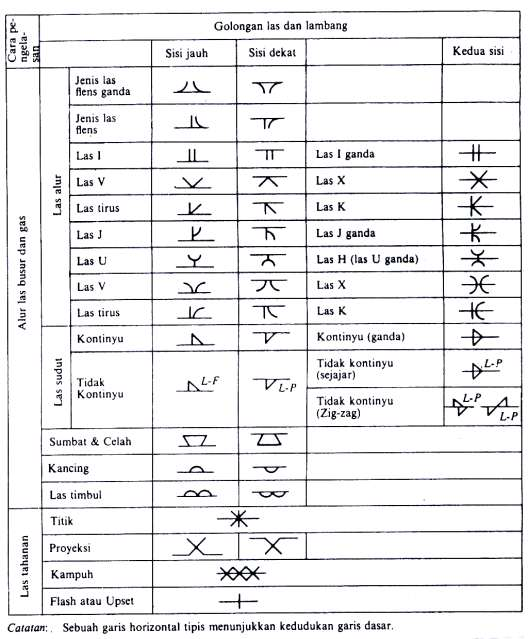
\includegraphics[width=.82\textwidth]{../figures/lambang_las.jpeg}
		% filename may not contain space but _
	\end{center}
	\caption{Lambang-lambang Las}
	\label{fig:lambang_las}
\end{figure}

Untuk menjelaskan penggunaan dari lambang-lambang las di atas, berikut ini disajikan beberapa contoh penggunaannya. Tabel~\ref{fig:penggunaan_las} menyajikan penggunaan lambang-lambang las tersebut.


\begin{figure}
	\begin{center}
		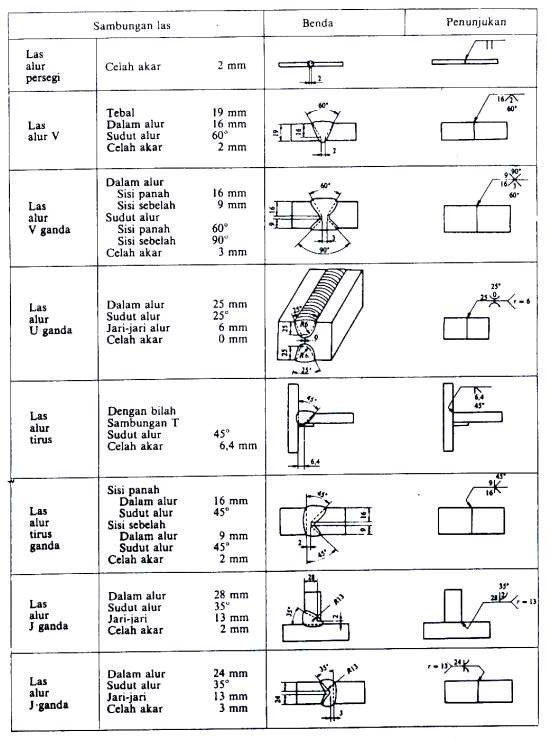
\includegraphics[width=.82\textwidth]{../figures/penggunaan_las.jpg}
		% filename may not contain space but _
	\end{center}
	\caption{Contoh Penggunaan Lambang-lambang Las}
	\label{fig:penggunaan_las}
\end{figure}














\bibliographystyle{apalike}
\bibliography{../filename.bib} % required for citecompletion, not work in mainfile
\end{document}

